\chapter{Varietà}


\section{Varietà topologica}

\begin{definition}
	Un $(X,\tau)$ spazio topologico, è detto \textbf{localmente euclideo} se per ogni $x \in X$ esiste $n \in \N$ e $U_x \subset X$ intorno aperto di $x$ tale che esiste un omeomorfismo $\morphism{\varphi_x}{U_x}{\mathring{\D}^n}$.  
\end{definition}

\begin{definition}
	Dato uno spazio topologico localmente euclideo, la coppia omeomorfismo intorno $(U_x, \varphi_x)$ è detta \textbf{carta locale}.
\end{definition}

\begin{remark}
	Dati due intorni distinti di $x$ per cui esiste una carta locale $(V_x, \varphi_x)$ e $(U_x, \psi_x)$, allora entrambi gli omeomorfismi avranno come codominio uno stesso $\mathring{\D}^n$ dove $n$ è uguale per entrambe le carte. (È un teorema profondo come un pozzo che non verrà trattato in queste note)
\end{remark}

\begin{theorem}
	Il disco nella topologia euclidea $\mathbb{D}^n$ è connesso per archi. 
\end{theorem} 
\begin{proof}
	Dimostro che il disco è convesso e quindi connesso per rette (e in particolare per archi). Infatti sia 
	\begin{equation}
	\mathbb{D}^n := \{x\in \R^n\; |\; |x| \le 1\}
	\end{equation}
	allora basta far vedere che presi due punti vale che l'intera retta sta nel disco. Siano $x, y \in \mathbb{D}^n$ allora
	\begin{equation}
	|(1-t)x+ty| \le (1-t)|x| + t|y| \le 1-t+t =1
	\end{equation}
	per cui stanno tutti nel disco, segue immediatamente la tesi. 
\end{proof}

\begin{remark}
	Dal teorema precedente si può notare perché si è scelto in particolare $\mathbb{D}^n$ come insieme di riferimento per le carte locali. Infatti questo insieme è abbastanza semplice, con una topologia abbastanza conosciuta, e ha proprietà che non tutti i sottospazi di $\R^n$ hanno (per esempio $\left[0,1\right] \cup (2,3)$ non è omeomorfo al disco, non è compatto, non è neanche connesso).
\end{remark}

\begin{definition}
	Se $X$ è una varietà topologica $n$ è detta la sua dimensione locale in $x$ e viene indicata dalla funzione
	\begin{equation}
	\begin{aligned}	
	\dim_x	\colon & X \rightarrow \N \\
	& 	x	\mapsto n \\
	\end{aligned}
	\end{equation}
\end{definition}

\begin{definition}
	La funzione $\dim_x$ è continua in $\N$ dotato della topologia discreta in quanto localmente costante. Inoltre se $X$ è compatto $\dim_x(X)$ dev'essere connesso e nella topologia discreta gli unici connessi sono i singoletti. Pertanto $\dim_x$ è costante se $X$ connesso.
\end{definition}

\begin{corollary}
	Se $X$ localmente euclideo e connesso, allora $\dim_x = k$ per qualche $k \in \N$. $k$ viene detta dimensione reale di $X$.
\end{corollary}

\begin{theorem}
	Sia $X$ localmente euclideo, allora $X$ è connesso per archi. 
\end{theorem} 
\begin{proof}
	Fisso un $x \in X$ e definisco 
	\begin{equation}
	W_x := \{z \in X \;|\; z \sim x\}
	\end{equation}
	dove $\sim$ è la relazione di essere connessi per archi. Innanzitutto notiamo che: 
	se $z \in W_x$ allora anche l'intorno $U_z$ è connesso per archi poiché localmente euclideo (basta passare per l'omeomorfismo locale).\\
	
	Per cui supponiamo che $W_x \neq X$ allora deve esistere almeno un $y \in X$ tale che non è in $W_x$. Distinguiamo due casi: 
	\begin{enumerate}
		\item Se $U_y \cap W_x \neq \varnothing$ allora posso usare la seconda osservazione per concludere che anche $y \in W_x$ contro l'ipotesi originaria, quindi $W_x = X$.
		\item Se $U_y \cap W_x = \varnothing$ allora dev'essere che $U_y \subset W^c_x$. Poiché per ogni punto di $W^c_x$ vale che il suo intorno sta in $W^c_x$ (se no avrei la possibilità di collegarli per archi con $x$) e quindi $W^c_x$ è aperto e $W_x$ chiuso. Inoltre sempre per l'osservazione iniziale $W_x$ dev'essere aperto. Poiché $X$ connesso dev'essere che $W_x = \varnothing$ (ma è impossibile perché $x\in W_x$) o $W_x = X$, ovvero la tesi. 
	\end{enumerate}
\end{proof}


\begin{theorem}
	Se $X$ localmente euclideo allora le sue componenti connesse sono aperte e chiuse.
\end{theorem}
\begin{proof}
	Se $X$ è connesso allora ha una sola componente connessa e quindi è sia chiusa che aperta.
	Sia $X$ sconnesso allora prendo una componente connessa $\left[x\right]_\sim$. Osservo che $\pi^{-1}(\left[x\right]_\sim)$ è un aperto: prendo un intorno $U_x \simeq \mathbb{D}^n$ per qualche $n$ e questo è connesso, per cui per ogni punto $x \in U_x \subset \pi^{-1}(\left[x\right]_\sim)$. Inoltre $\pi(\pi^{-1}(\left[x\right]_\sim)) = \left[x\right]_\sim$ per suriettività. Inoltre anche $\pi^{-1}(\left[x\right]^c_\sim)$ è aperto, infatti se fosse chiuso avrei che per ogni $y$ sulla frontiera questo sarebbe connesso con $x$, il ché sarebbe assurdo. Quindi $\left[x\right]_\sim$ è sia aperto che chiuso in $\tau_\sim$.
\end{proof}

\begin{remark}
	In generale se uno spazio topologico è localmente euclideo non è di Hausdorff. Infatti si consideri $\{a,b\} \times \R$ con la relazione di equivalenza $(x,y) \sim (z,w) \leftrightarrow y = w \land y \ge 0 \lor (x,y) = (z,w)$. Allora il disegno diventa una sorta di Y, in cui dove le due rette si congiungono c'é lo 0.
	\begin{figure}[h]
		\centering
		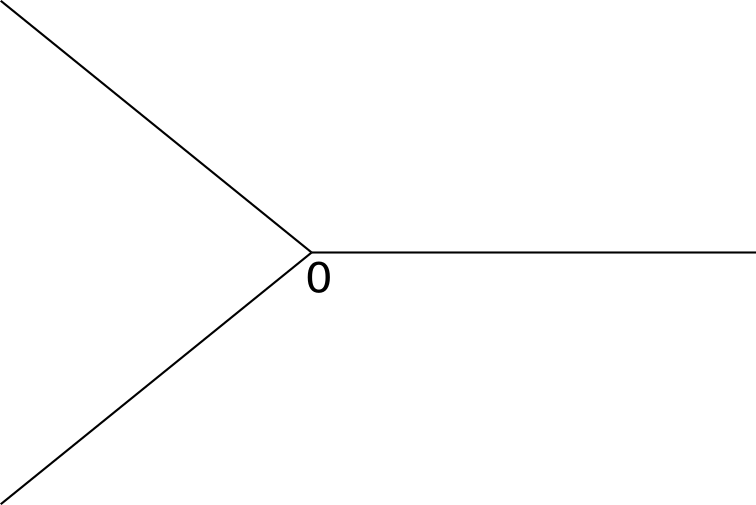
\includegraphics[width=0.35\linewidth]{images/topologia_generale/lcleucnott2}
		\caption{}
		\label{fig:lcleucnott2}
	\end{figure}
	
	Questo spazio è localmente euclideo, ma non è di Hausdorff.
\end{remark}

\begin{definition}
	Uno spazio topologico $(X,\tau)$ è detto \textbf{varietà topologica} di dimensione $n$ se è localmente euclideo, connesso, di Hausdorff e a base numerabile.
\end{definition}

\textbf{Alcuni esempi}

\begin{enumerate}
	\item Per $n=1$ le uniche varietà topologiche sono $\S^1$ e $\R$.
	\item Per $n=2$ le varietà topologiche si chiamano superfici topologiche e sono \textit{troppe}.
	\item Il toro si può costruire come $\left[0,1\right]^2/\Z^2$ si vede che è localmente euclideo, di Hausdorff, connesso e a base numerabile ed è anche compatto. Il toro è anche un esempio di superficie non orientabile e questo è di grande importanza nella teoria dei modelli minimali. Infatti grazie al toro è possibile generare tutte le superfici topologiche non orientabili. In generale il toro si indica con $T_g$ dove $g$ indica quante volte è stato aggiunto a  se stesso. Ad esempio un toro semplice si indica con $T_1$, mentre un bitoro $T_2$, mentre $T_0$ equivale alla sfera (più che altro per semplificare la notazione dei teorem, visto che è un caso limite).
	\item Anche il piano proiettivo si può esprimere come $\S^2 / \sim$ dove $a \sim b \Leftrightarrow a = rb$ per qualche $r \in \R$. Ma quest'ultimo si può vedere che è omeomorfo a $\D^2$. Pertanto $\mathbb{P}^2(\R) \simeq \D^2$. Il piano proiettivo viene denominato anche $U_n$ dove $n$ rapprensenta il numero di volte che viene sommato a se stesso, ovvero $U_1 + \dots + U_1 = U_n$.
\end{enumerate}

\begin{definition}[Somma connessa]
	Date due varietà topologiche $V_1, V_2$ è possibile trovare un intorno di $V_1$ e $V_2$ tali che sono omeomorfi (passando per la proiezione sul disco euclideo), per cui collegando le rispettive frontiere è possibile \textit{attaccare} $V_1$ con $V_2$. In particolare questa operazione si indica con $V_1 + V_2$ ed è indipendente dalla scelta dell'intorno a meno di omeomorfismi. 
\end{definition}


\begin{theorem}[Teorema di classificazione]
	Ogni superficie topologica compatta è omeomorfa a un $T_g$ per qualche $g \ge 0$ e $U_h$ per qualche $h \ge 1$, inoltre i due modelli non sono omeomorfi e sono minimali. 
\end{theorem}

L'intuizione di ciò è data dal fatto che il toro può essere rappresentato dalla stringa $aba^{-1}b^{-1}$ e il piano proiettivo da $aa$, mentre la sfera da $aa^{-1}$, per cui tutte le possibili stringhe sono di questo tipo visto che la somma connessa risulta essere, in questo caso, una semplice concatenazione di queste stringhe. La dimostrazione della minimalità verrà data nella prossima sezione.


\section{Classificazione superfici compatte}

Per poter classificare le superfici abbiamo bisogno di alcuni strumenti algebrici sui gruppi. In particolar modo il calcolo degli abelianizzati e dei gruppi dei nostri modelli fondamentali: il toro e il piano proiettivo.

\begin{lemma}
	\label{lemm:abel_torus_proj}
	Valgono i seguenti isomorfismi di gruppi
	\begin{equation}
	\begin{aligned}
	 Ab(\pi_1(U_h, x_0)) & \simeq \Z^{h-1} \times \Z_2 \\
	 Ab(\pi_1(T_g, x_0)) & \simeq \Z^{2g}
	\end{aligned}
	\end{equation}  
\end{lemma}
\begin{proof}[1]
	Sappiamo che $\pi_1(U_h) \simeq \left\langle \alpha_1, \dots, \alpha_h \mid \alpha^2_1 \cdots \alpha^2_h = 1\right\rangle$, quindi abelianizzando il gruppo si ottiene (utilizzando le trasformate di Tietze)
	\begin{equation}
	\begin{aligned}
		& Ab( \left\langle \alpha_1, \dots, \alpha_h \mid \alpha^2_1 \cdots \alpha^2_h = 1\right\rangle) \\
		& \simeq \left\langle \alpha_0, \alpha_1, \dots, \alpha_h \mid \alpha^2_1 \cdots \alpha^2_h = 1,\ \alpha_0 = \alpha_1 \dots \alpha_h,\ \left[a_i, a_j\right],\ \forall i,j \right\rangle\\
		& \simeq \left\langle \alpha_0, \alpha_1, \dots, \alpha_h \mid \alpha^2_0 = 1,\ \left[a_i, a_j\right],\ \forall i,j \right\rangle \\
		& \simeq \left\langle \alpha_1, \dots, \alpha_h \mid \left[a_i, a_j\right],\ \forall i,j \right\rangle \times \left\langle \alpha_0 \mid \alpha^2_0 = 1\right\rangle \simeq \Z^{h-1} \times \Z_2 
	\end{aligned}
	\end{equation}
\end{proof}
\begin{proof}[2]
	Sappiamo che $\pi_1(T_g) \simeq \left\langle \alpha_1, \dots, \alpha_g, \beta_1, \dots, \beta_g \mid \alpha_1 \beta_1\alpha^{-1}_1\beta^{-1}_1 \dots \alpha_g \beta_g\alpha^{-1}_g\beta^{-1}_g = 1\right\rangle$. Quindi la relazione sui generatori coincide al prodotto di tutti i commutatori, per cui 
	\begin{equation}
	\begin{aligned}
		& Ab(\left\langle \alpha_1, \dots, \alpha_g, \beta_1, \dots, \beta_g \mid \alpha_1 \beta_1\alpha^{-1}_1\beta^{-1}_1 \dots \alpha_g \beta_g\alpha^{-1}_g\beta^{-1}_g = 1\right\rangle) \\ & \simeq \left\langle \alpha_1, \dots, \alpha_g, \beta_1, \dots, \beta_g \mid \left[\alpha_1, \beta_1\right] = \dots \left[\alpha_g \beta_g\right] = 1\right\rangle\\
		& \simeq \left\langle \alpha_1 \mid \varnothing \right\rangle \times \dots \times \left\langle\beta_g \mid \varnothing \right\rangle \simeq \Z^{2g}
	\end{aligned}
	\end{equation}
\end{proof}

\begin{definition}
	Sia $G$ un gruppo abeliano; un elemento $g \in G$ si dice di torsione se per qualche $n \in \N$ vale $ng = 0$. L'insieme degli elementi di torsione forma il sottogruppo $T(G) \subset G$.
\end{definition}

\begin{lemma}
	Siano $G, G'$ gruppi abeliani. Allora valgono i seguenti fatti
	\begin{enumerate}
		\item Se $\morphism{\varphi}{G}{G'}$ è un morfismo tra gruppi, allora vale $\varphi(T(G)) \subseteq T(G')$.
		\item Se $\varphi$ come definito sopra è un isomorfismo, allora $\varphi|_{T(G)}$ un isomorfismo sui sottogruppi di torsione.
		\item Inoltre se $\varphi$ è un isomorfismo di gruppi, allora induce un isomorfismo $\morphism{\overline{\varphi}}{G/T(G)}{G'/T(G')}$.  
	\end{enumerate}
\end{lemma}

\begin{proposition}
	$\Z^n \simeq \Z^m$ se e solo se $m = n$. 
\end{proposition}
\begin{proof}
\end{proof}

\begin{theorem}
	Sia $S$ una superficie compatta. Allora essa è omeomorfa a $T_g$ con $g\ge 0$ oppure ad una superficie $U_h$ per $h > 0$. Inoltre $T_g \not\simeq U_h$ per ogni $g,h$, $U_h \not\simeq U_{h'}$ per $h\neq h'$ e $T_{g'} \not\simeq T_g$ per $g \neq g'$.
\end{theorem}
\begin{proof}
	Il fatto che $S$ sia omeomorfa ad una delle due superfici è già stato dimostrato. Non resta che dimostrare la minimalità dei modelli presi.\\
	
	\textbf{$T_g \not\simeq U_h$}\\
	
	Consideriamo gli abelianizzati dei gruppi fondamentali rispettivi. Per il Lemma \ref{lemm:abel_torus_proj} vale che 
	\begin{equation}
	\begin{aligned}
		Ab(\pi_1(U_h, x_0)) & \simeq \Z^{h-1} \times \Z_2 \\
		Ab(\pi_1(T_g, x_0)) & \simeq \Z^{2g}
	\end{aligned}
	\end{equation}
	che hanno rispettivamente come sottogruppo di torsione $\Z_2$ e $\{0\}$, quindi non possono essere isomorfi ed in particolare non $T_g \not\simeq U_h$ (inoltre non sono neanche omotopicamente equivalenti).
	
	\textbf{$U_h \not\simeq U_{h'}$} \\
	
	Se fossero isomorfi allora gli abelianizzati sarebbero isomorfi e inoltre il quoziente dell'abelianizzato per il sottogruppo di torsione sarebbe isomorfo. In particolare 
	\begin{equation}
	\begin{aligned}
		\Z^{h-1} \simeq \Z^{h-1} \times \Z_2 / \Z_2 \simeq \Z^{h'-1} \times \Z_2 / \Z_2 \simeq \Z^{h'-1}
	\end{aligned}
	\end{equation}
	che funziona se e solo se $h = h'$.
	
	\textbf{$T_g \not\simeq T_{g'}$} \\
	
	Se fossero isomorfi allora gli abelianizzati sarebbero isomorfi quindi valrebbe $\Z^{2g} \simeq \Z^{2g'}$ che è valido solo se $g = g'$.
\end{proof}


% TODO: Inserire esempi da minuto 22 della lezione del 24/03/2020.
\textbf{Esempi e osservazioni sui retratti}\\
